\section{Introduction}
\label{sec:introduction}

% General introduction
This tutorial helps you learn to use PFunc, short for Parallel Functions, a
lightweight and portable library that provides C and \Cpp{} APIs to express
task parallelism. 
%
PFunc enables programmers to focus on developing parallel algorithms and
specify low-level and high-level tasks to parallelize instead of working with
native threading libraries such as POSIX and Windows threads.
%
Although there are several task libraries, PFunc is unique in that its features
are a strict superset of the features offered by current solutions for task
parallelism.  
%
Specifically, PFunc extends the feature set of current solutions with custom
task scheduling, task priorities and task affinities.
%
In addition, PFunc offers task groups for SPMD-style programming and multiple
task completion notifications for parallel execution of DAGs. 
%
PFunc's extended feature set is geared towards helping knowledgeable users
optimize their application performance. 
%

\subsection{Organization}
\label{subsec:organization}
%
\begin{figure}[t]
\centering
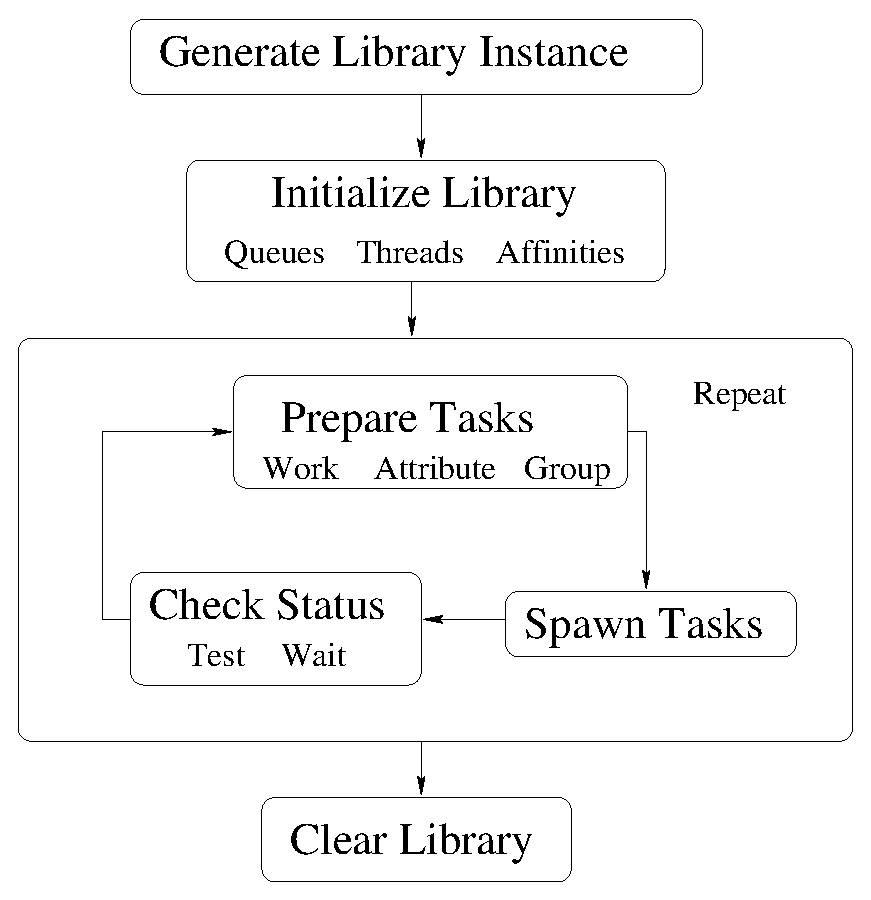
\includegraphics[width=0.5\textwidth]{figs/life-cycle}
\caption{Life-cycle of a PFunc application.}
\label{fig:life_cycle}
\end{figure}
%
Figure~\ref{fig:life_cycle} depicts the life-cycle of a PFunc
application. 
%
First, the library is initialized. Then, tasks are repeatedly spawned and
executed in parallel.  Finally, the library instance is cleared.
%
This tutorial is organized to reflect the life-cycle of PFunc applications.
%
The table below gives a brief summary of each section.
% 
\begin{center}
\begin{tabular}{|c|l|}
\hline
Section & Explanation \\
\hline
Section~\ref{sec:introduction} & Introduction to the tutorial.\\
\hline
Section~\ref{sec:install} & Installation and package information.\\
\hline
Section~\ref{sec:generate} & Generating PFunc's library instance description.\\
\hline
Section~\ref{sec:initialize} & Initializing the library.\\
\hline
Section~\ref{sec:spawn} & Creating, spawing, and waiting for tasks.\\
\hline
Section~\ref{sec:fibonacci} & A complete Fibonacci example in C. \\
\hline
Section~\ref{sec:pack} & Packing and unpacking arguments in C. \\
\hline
Section~\ref{sec:attribute} & Setting task attributes. \\
\hline
Section~\ref{sec:group} & Group operations in PFunc.\\
\hline
Section~\ref{sec:sync} & Locks and atomic operations.\\
\hline
Section~\ref{sec:loops} & Higher-level parallel loop primitives.\\
\hline
Section~\ref{sec:exception} & Handling exceptions.\\
\hline
Section~\ref{sec:perf} & Gather hardware statistics using PFunc and PAPI.\\
\hline
Section~\ref{sec:design} & A detailed description of PFunc's design.\\
\hline
Section~\ref{sec:custom} & Customizing PFunc. \\
\hline
\end{tabular}
\end{center}

\subsection{Salient Features}
\label{subsec:salient}
%
\paragraph{Customizable}
%
PFunc can be used ``out-of-the-box''; however, for the more adventerous users,
most of PFunc's features are completely customizable.
%
PFunc is the first task parallel library to offer STL-like customization of
task scheduling policy, task stealing policy, task priorities, and task
affinities.
%
As a result, PFunc is a great fit in an academic environment.

%
\paragraph{Generic}
%
PFunc is unique in its heavy use of generic programming --- a programming
paradigm for developing efficient and reusable software libraries.
% Continued
While developing PFunc, we applied the process of ``lifting'' to find both
commonality and missing features among existing task parallelism
implementations such as Cilk, Intel's Threading Building Blocks, and OpenMP
tasks.
%
The use of generic programming allows PFunc to be flexible and yet highly 
efficient as most of its customizations are done at compile-time.

%
\paragraph{Task parallelism}
%
PFunc provides a super-set of the features offered by other task parallel
solutions.
%
For example, it introduces the ability to deliver multiple task completion
notifications and the notion of task groups.
%
Multiple task completion notifications allow users to execute arbitrary DAG 
computations instead of the traditional tree-based model supported in most 
other solutions.
%
On the other hand, groups allow users to seamlessly incorporate SPMD-style
semantics into their task parallel algorithms.

%
\paragraph{Loop parallelism}
%
A vast majority of algorithms can be parallelized by merely parallelizing the 
loops in these algorithms.
%
PFunc offers three high-level parallel loop structures: \code{for},
\code{while}, and \code{reduce}, which can be used without delving into the
details of task parallelism. 

%
\paragraph{Production-grade}
%
Finally, PFunc provides production-grade exception handling and performance
monitoring mechanisms to assist software developers.
